\chapter{基于应用场景的系统层能效优化}

本章首先介绍了动态电压频率调节(DVFS)的基本概念以及其在能效优化领域所发挥的作用。本章利用前述章节所实现的CNN运行时库开发了一款智能监控系统Android应用。\ref{chapter5-2}节对该应用的负载特征进行了刻画与分析,阐述了当前Android系统所采用的功耗管理器在基于深度学习模型应用上表现的不足之处。\ref{chapter5-3}节提出了一种基于应用场景的系统层能效优化策略,该策略根据应用在系统层表现的负载特征对其进行分类,这样系统便可以针对不同的应用使用不同的功耗管理策略。

\section{动态电压频率调节技术}

动态电压频率调节DVFS(Dynamic Voltage and Frequency Scaling)是一种可对芯片电压和频率进行实时动态调节的技术。当前手机CPU和GPU都支持DVFS,并且系统层也都存在着相应的功耗管理器(governor)。每一个功耗管理器都拥有一个执行频率调节的策略,并且这个策略可被配置以取得不同的能效折中。根据配置的策略,功耗管理器可以决定不同状态下的设备处理器所应该运行的频率。设备处理器的负载越高运行频率越高是这些功耗管理器所遵循的基本准则。

动态功耗\cite{benini1999policy}、短路功耗\cite{周宽久2010嵌入式软硬件低功耗优化研究综述倡}和漏电流功耗\cite{you2006compilers}是CMOS电路的三个主要功耗,因此CMOS电路的总功耗可由公式\ref{equation:equation3}表示:

\begin{equation}
     \label{equation:equation3}
     \begin{aligned}
        P = P_{Dynamic} + P_{Short} + P_{Leakage}
         = ACV^2f +  AVI_{Short} + VI_{Leakage}
     \end{aligned}
\end{equation}

式中$C$代表负载电容的容值,$V$是工作电压,$A$是当前频率下电路的平均翻转率,$f$为工作频率,$I_{Short}$和$I_{Leakage}$分别为短路电流和漏电流。从公式中可知,$C$、$V$、$A$、$f$决定了整个CMOS电路的功耗,而DVFS技术就是主要通过改变频率$f$和电压$V$的值来调节系统功耗的。


\section{智能监控系统Android应用的负载特征}
\label{chapter5-2}

基于前述章节所实现的CNN运行时库,本文开发了一款智能监控系统Android应用,其可以通过手机摄像头自动辨识周围所观察到的物体类别。图\ref{figure:figure31}显示了两张该应用的运行界面。智能监控系统应用的智能识别功能是由卷积神经网络Tiny YOLO\cite{pjreddie.com}卷积模型提供的。

\begin{figure}[htbp]
    \centering
    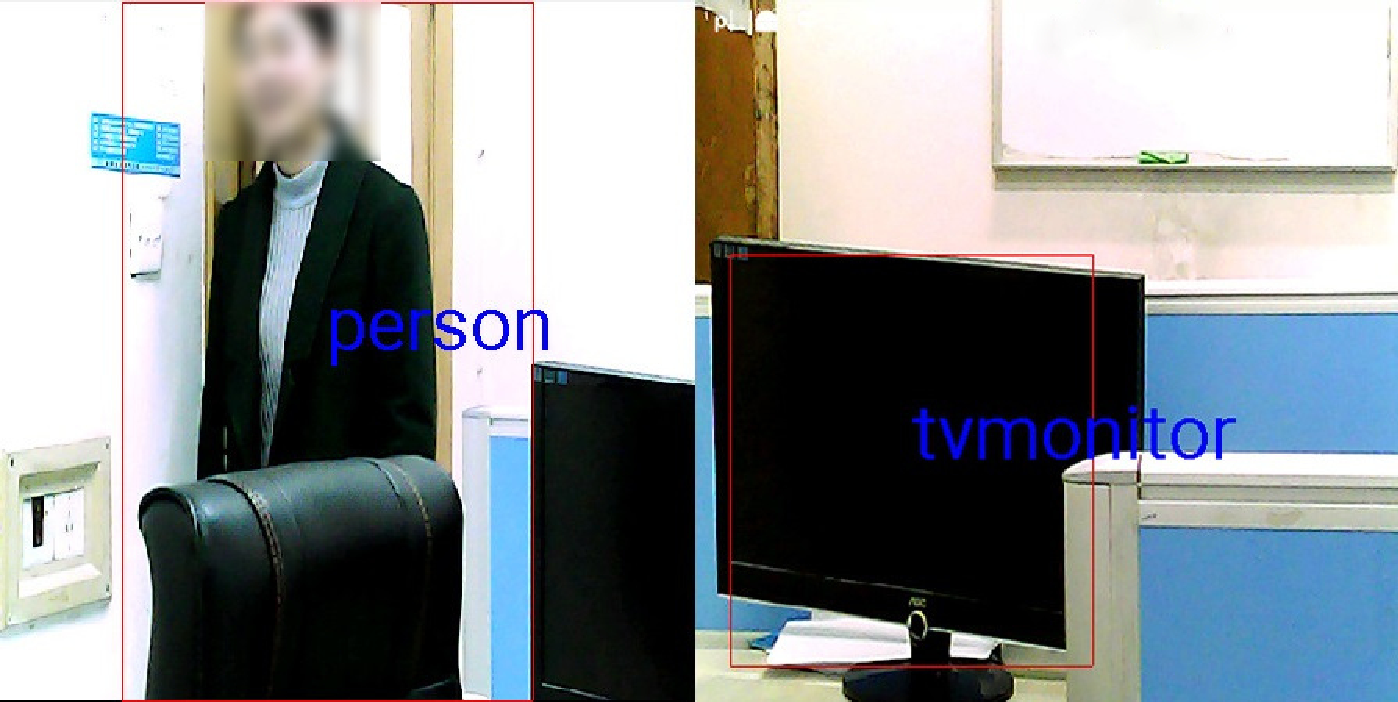
\includegraphics[height=0.4\textwidth]{figures/app.pdf}
    \caption{智能监控系统Android应用}\label{figure:figure31}
\end{figure}

图\ref{figure:figure36}显示了智能监控系统Android应用的工作流程。在智能监控系统APP启动后,它会不断地通过手机摄像头感知周围的场景。当读取到摄像头所拍摄视频中的一帧数据后,该APP会立即将该帧数据作为CNN模型的输入并执行网络的前向推断过程。推断完成后,侦测结果会在视频框中显示出来。紧接着,监控APP会立即获取下一帧图像数据并重复上述过程。

\begin{figure}[htbp]
    \centering
    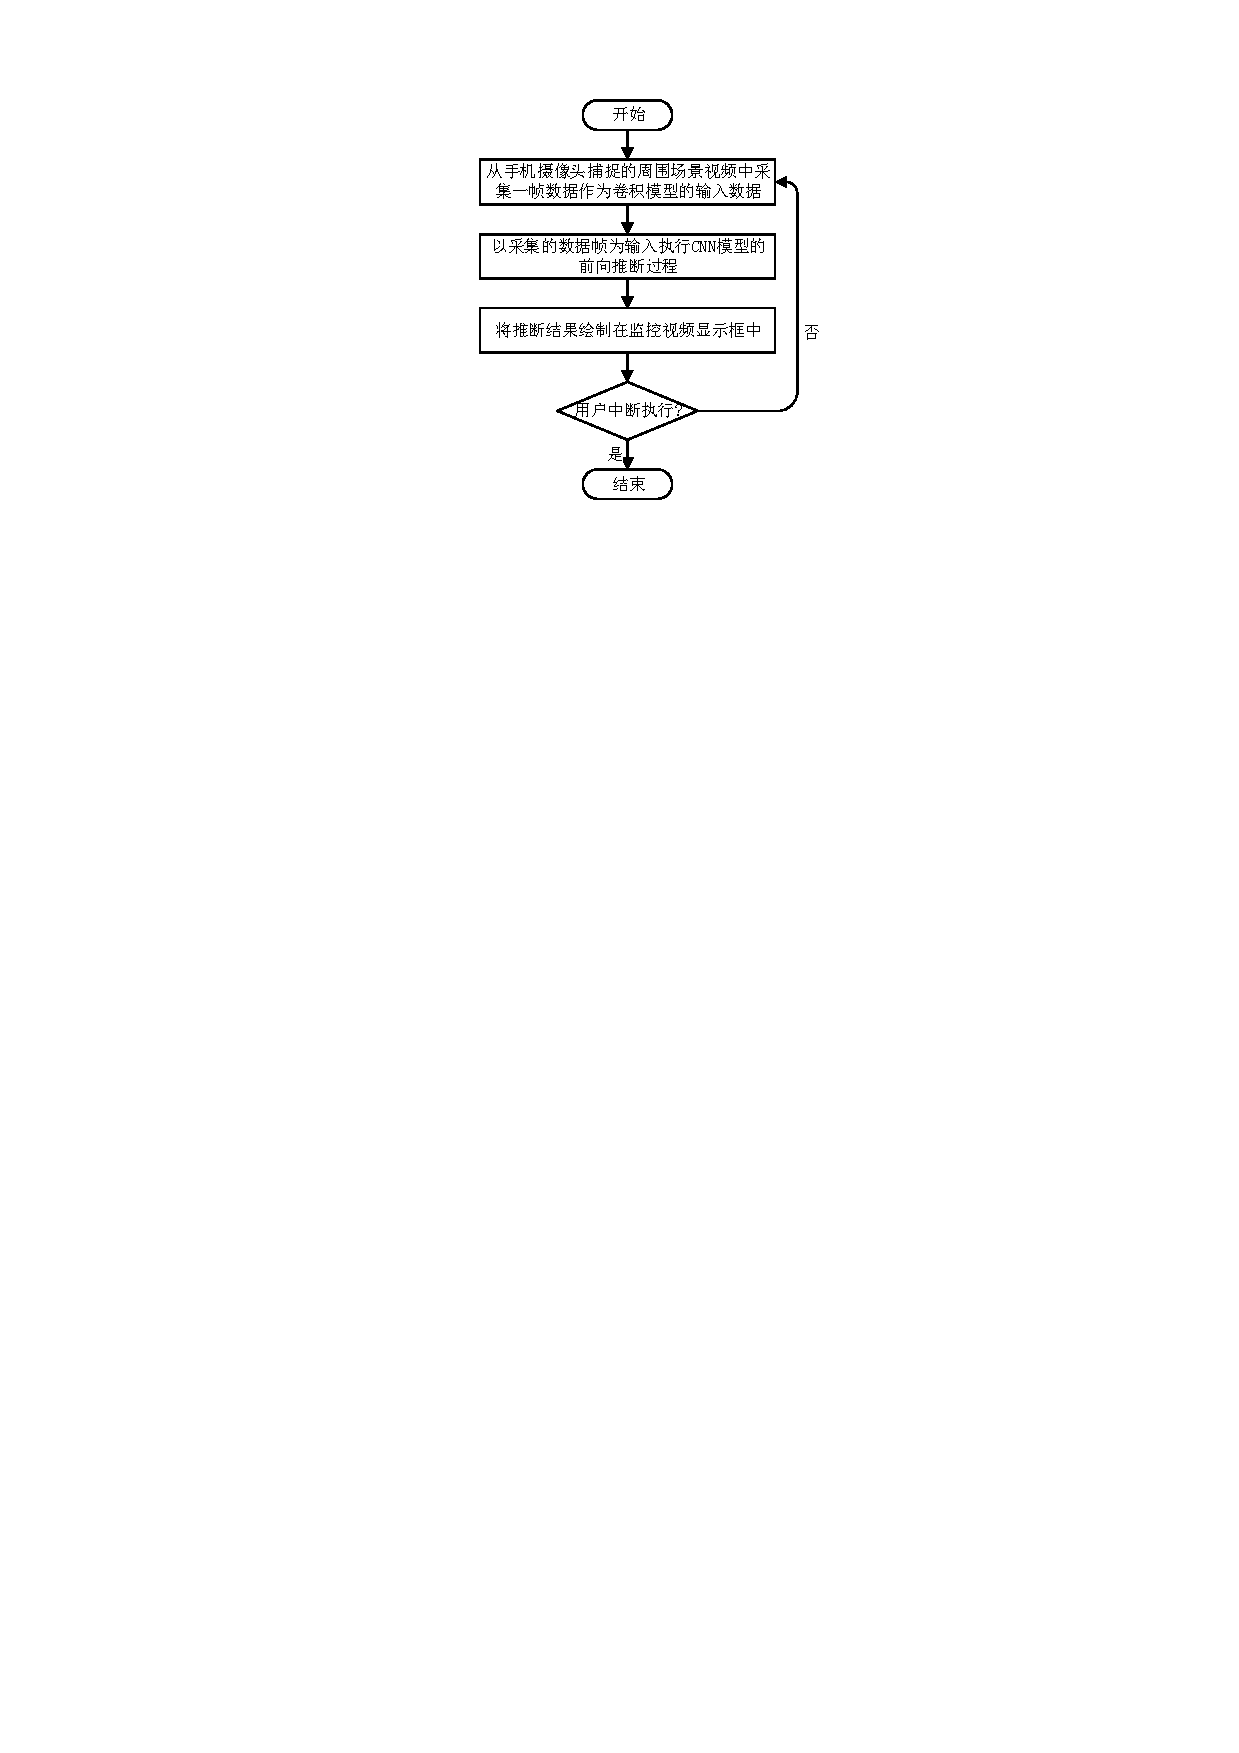
\includegraphics[height=0.5\textwidth]{figures/app_process.pdf}
    \caption{智能监控系统APP的工作流程}\label{figure:figure36}
\end{figure}

为了探索从系统层进一步优化基于CNN模型的手机应用,本文基于ODROID-XU3平台考察了智能监控系统APP的运行时负载特征。由第\ref{chapter:chapter4}章可知,智能监控系统APP在ODROID-XU3上主要使用GPU执行CNN的前向推断过程,故而可使用GPU的利用率作为该APP的负载。图\ref{figure:figure37}显示了在Android系统GPU默认功耗管理策略下智能监控系统APP的负载和GPU频率变化情况。
由图\ref{figure:figure37}可以看出,智能监控系统APP对GPU的利用率平均值为86.59\%,并且绝大多数的利用率值都在平均线以上。智能监控系统APP的负载曲线形状类似了周期脉冲图,这与该APP的实际工作流程相符合。因为智能监控系统APP的工作流程就是周期性的“采样-推断-绘制”。由智能监控系统APP的负载曲线上只有一个很窄的峰谷可知,“采样-推断-绘制”操作中推断占了整个APP运行时间的绝大部分。
\begin{figure}[htbp]
    \centering
    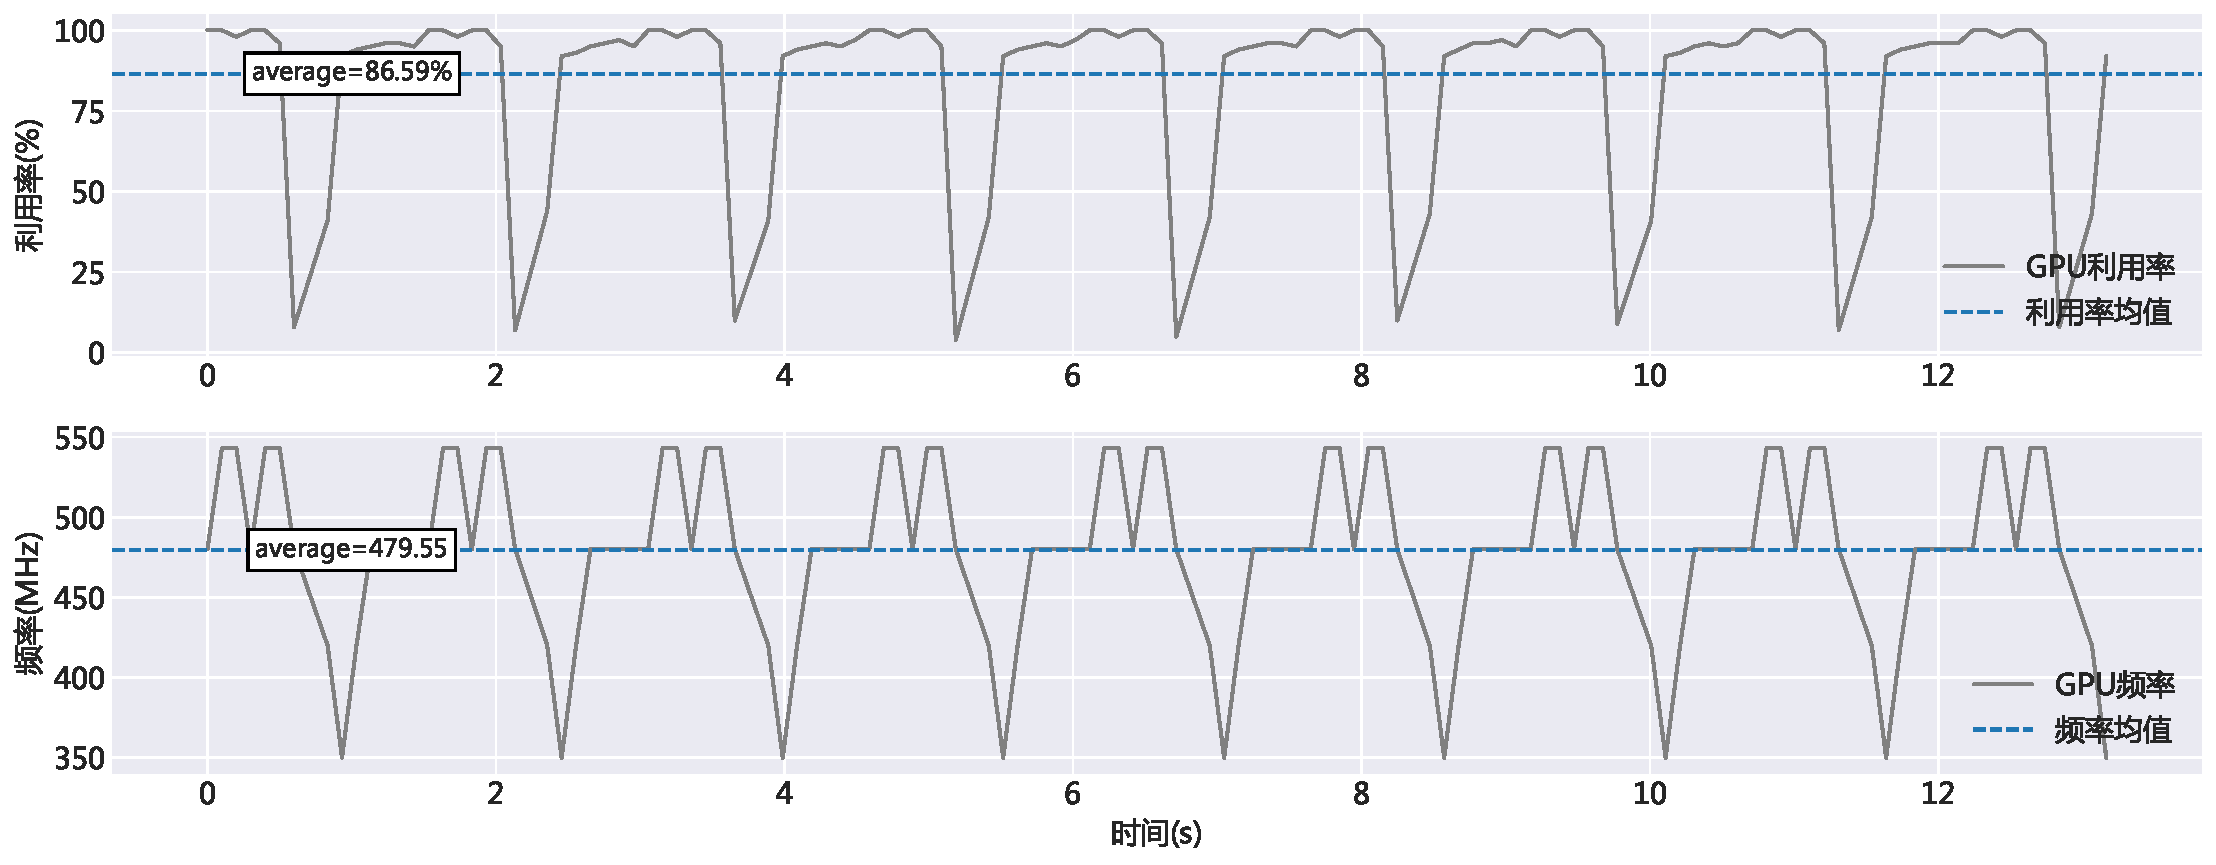
\includegraphics[width=1.0\textwidth]{figures/system_util.pdf}
    \caption{智能监控系统APP的负载和GPU频率变化}\label{figure:figure37}
\end{figure}




\section{基于应用场景的系统层能效优化策略}
\label{chapter5-3}

\section{本章小结}


\cleardoublepage